\section{Enrichment Overview}
% Paper 2
The term enrichment in this context describes the extension of the (semantic)
schema of a knowlege base. The process of knowlege base enrichment increases the
semantic richness and the expressiveness of the knowlege base. 
The goal of the enrichment progress is to find axioms, witch can be added to the
existing ontology. A special case is to find definition of classes and
subclasses. This is closely related to the Inductive Logic Programming (ILP) as
it is described later in this article.
Ontology enrichment methods usually depend on machine learning or on applying
heuristics to find additional axioms in the knowlege graph.\cite{paper2}

As stated before, knowlege base enrichment usually work on existing data to
improve the semantic schema. This supports the so called \emph{grass-root}
approach for creating ontologies. Here whole ontologie structure is not created
upfront, but evolves over time and with every part of data that is added to the
knowlege base.\cite{paper2}

% Liste approaches
- description logic: least common subsumer
- top-down, refinement operator for ALER 
- combine in YINYANG tool 

% Paper2: p60
- knowlege base completetion (well-defined sense) classes <-> subclasses 

- CELOE (heuristics and adaptation), described later

\begin{figure*}
\centering
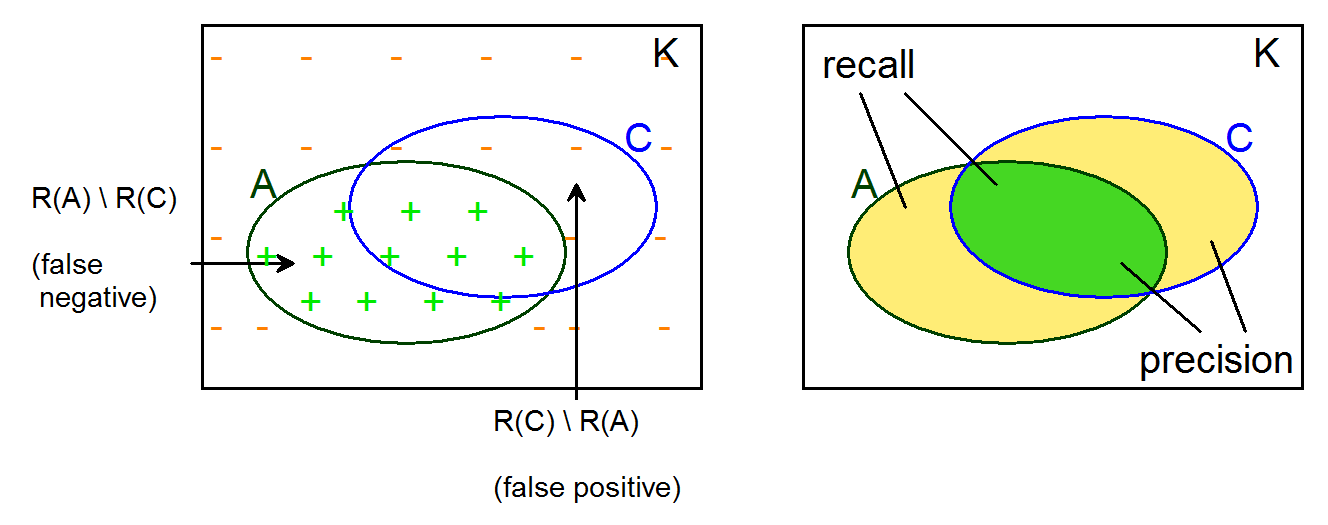
\epsfig{file=img/venn.png, width = 14 cm}
\caption{recall precision}
\end{figure*}



%=====================================================================================
%=====================================================================================
%=====================================================================================
\section{Class Learning}
% Paper 1
\subsection*{Motivation}
The class learning approach is one method of enrichment of knowlege bases. It
aims at finding new definition of classes to extend the semantic schema. For the
motivation of the method consider the following example.

\newdef{example}{Example}
\begin{example}
For this example consider a knowlegde base containing a class \emph{President of
the United States} with instance data like Abraham Lincoln, John F. Kennedy,
Bill Clinton and Barack Obama. A class Learning algorithm may suggest that the
President class is equivalent to the following two class expressions:
\\\hspace*{12pt}\texttt{Person and born in the USA}\\
\hspace*{12pt}\texttt{American citizen and born in the USA}\footnote{The class
'American citizen' is here a subclass of 'Person', witch makes the second
statement more specific.}
\end{example}

These suggestions would then be presented to a knwolege engineer who than can
decide if they are plausible and should be added to the knowlege graph. Should
the engineer for instance choose the second statement he could check if there
are instances of the class president, where the individual is not of type
American citizen. This could indicate an error or missing information in the
knowlege graph witch could be fixed by this semi-automated approach by the
knowlege engineer.


\subsection*{Learning Problem}
The problem of learning class definitions for given data depend on the so called
inductive reasoning as opposed to inference or deductive reasoning. \cite{paper1}
Inductive Reasoning is also a key concept in Inductive Logic Programming.

\newdef{definition}{Definition}
\begin{definition}
We are searching for a formal description of the class $A$, which has existing
instances in the examined ontology. A possible class expression $C$ then
contains axioms of the form $A \subseteq C$ or $A \equiv C$.
\end{definition}

This means that the learned expression $C$ is a description of the individuals
of $A$. In our president example, the individuals are the presidents John F.
Kennedy, Barack Obama etc. whereas $C$ can be one of the suggested expression.
In many cases there will be no exact solution for $C$, but rather an
approximotion. This can be the case, if the knowlege base contains false class
assignments or missing information. In our example the birthplace of Thomas
Jefferson might be missing in the ontology. However, if most of the other
presidents have the correct birthplace the learning algorithm may still suggest
the expressions. Again, missing information may be completed by the knowlege
engineer.

In a complexe knowlege base a class learning algorithm may find many new class
definition and often different expression for the same class. Based on Occam's
razor \cite{occam-razor} simple solutions are preferred over complex ones,
because they are more readable an thus easier for the knowlege engineer to
evalueate. Simplicity is measured in an straight forward way: the lenght of an
expression, which consists of role, concept and quatifiers.
The algorithm is biased towards shorter expressions. \cite{paper1}

\subsection*{Algorithm}
One algorithm for solving the learning problem is called CELOE (Class
Expression Learning for Ontology Engineering). It is described in \cite{paper1}.
An brief overview of CELOE is given in Figure 2.
\begin{figure}
\label{celoe}
\centering
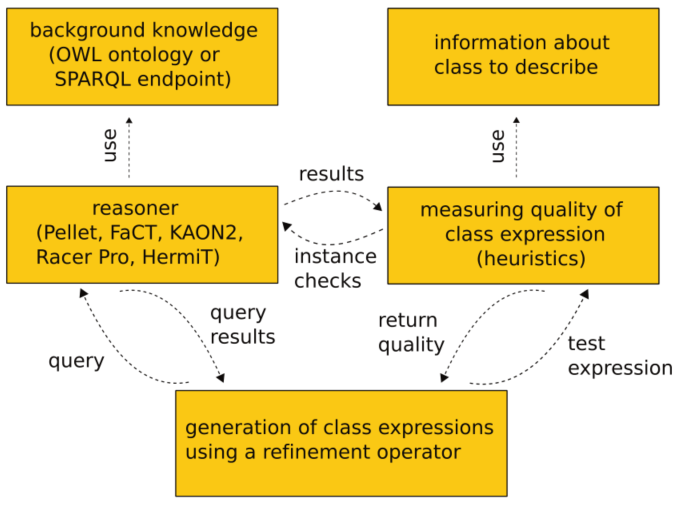
\epsfig{file=img/celoe.png, width = 8 cm}
\caption{CELOE\cite{paper1}}
\end{figure}
The algorithm follows the ``generate and test'' approach which is the common
concept in ILP. 
In the learning process many class expression are created and tested against the
background knowlege. Each of these class expressions is evalued using diffenrent
heuristics, which are described in detail in a separate section.

To find appropiate class expression to describe existing classes CELOE uses a so
called \emph{refinement operator}. The idea of these operator is based on the
work in \cite{refinement1},\cite{refinement2} and \cite{refinement3}. Refinement
operators are used to search in the space of expressions. It can be seen as a
top-downl algorithm as it is illustrated in Figure 3.
As an example consider the following path ($\leadsto$ indicates a refinement
step):\vspace{6pt}\\
$T \leadsto Person \leadsto Person \sqcap takesPartIn.T \leadsto Person \sqcap
takesPartIn.Meeting$

\begin{figure}
\label{tree}
\centering
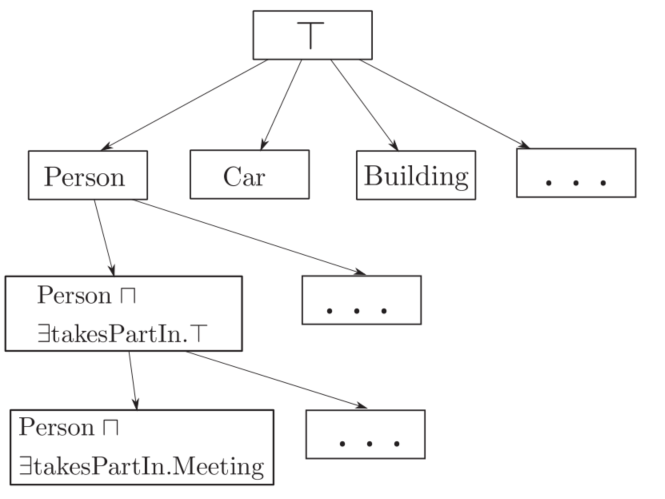
\epsfig{file=img/tree.png, width = 8 cm}
\caption{Tree\cite{paper1}}
\end{figure}

%=====================================================================================
%=====================================================================================
%=====================================================================================
\section{Enrichment with OWL Axioms}
% Paper 2
OWL offers many different types of axioms for a method to enrich the knowlege
base. 
\begin{figure}
\label{3-Phase}
\centering
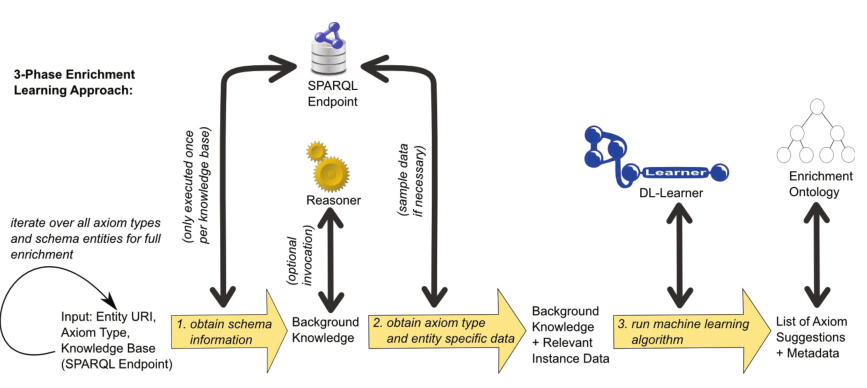
\epsfig{file=img/3-phase-enrichment.png, width = 8 cm}
\caption{3-Phase Enrichment Workflow\cite{paper2}}
\end{figure}
Figure \ref{3-Phase} shows the 3 steps in the enrichment workflow as described
in \cite{paper2}:
\begin{enumerate}
  \item The first phase is about obtaining general information about the
  knowlege base, in particular axioms, which define the class hierarchy are
  obtained. The schema queried via SPARQL, but is loaded only once.
  \item In the second phase data is again obtained via SPARQL. These background
  checks allows the method to learn and test new axioms. Examples for axiom
  types are explained in the following text.
  \item The score of axiom candidates is computed and the result is returned.
\end{enumerate}

The algorithm for suggestion of new axioms is based on checking and counting RDF
triples. In the following example we want to learn if the class $A$ is an
appropiate domain of a predicate $p$. For that we count the triples that match
this statement to obtain a score. 

\begin{example}
Lets look at the predicate \texttt{onto:attendsMeeting} and check if we can find
a suitable candidate for a domain. Note that \texttt{onto:Manager} is a subclass
of \texttt{onto:Employee}.
\end{example}
\begin{lstlisting}[morekeywords={onto, rdf, rdfs}, caption=Triples written in
turtle syntax] @PREFIX onto: <http://ontology-to-enrich.com/>.
onto:Software_Engineer		
		onto:attendsMeeting 	onto:TeamMeeting;
		rdf:type				onto:Employee.
onto:Software_Architekt		
		onto:attendsMeeting 	onto:TeamMeeting;
		rdf:type				onto:Employee.
onto:Project_Manager		
		onto:attendsMeeting 	onto:ManagerMeeting;
		rdf:type				onto:Manager.
		
onto:Manager   rdfs:subClassOf	onto:Employee.
\end{lstlisting}
Looking at this example we would abtain a score of 33.3 \% (1 out of 3) for the
class \texttt{onto:Manager} and 100 \% (3 out of 3) for the class
\texttt{onto:Employee}.\\
Obviously this extrem simple and straightforward method of calculating the score
for the domain of a predicate $p$ has some limitation.
Mainly the method doesn't discriminate between a score calculated by having 100
out of 100 correct observations or only 3 out of 3. Different methods, for
example the Wald method \cite{wald-methods}, overcome that problem. 
More involved heuristics are shown in the next section. 

\subsection*{Obtaining Axioms via SPARQL queries}
This section explains how SPARQL queries are used to extract information in step
2 of the enrichment workflow.

\subsubsection*{Subclass and Disjointness of classes}
This query evaluates all individuals (\texttt{?ind}) and checks if they are
instance of the user defined class definition in \texttt{\$class}. In this query
higher count indicates a better candidate for a superclass. 
Lower value indicates a disjointness.
 
\begin{lstlisting} 
SELECT ?type (COUNT(?ind ) AS ?count ) WHERE {
	?ind a <$class >.
	?ind a ?type .
} GROUP BY ?type
\end{lstlisting}

\subsubsection*{Subsumption and Disjointness of properties}
A pretty simular query can be used to learn subsumption and disjointness of
predicates.

\begin{lstlisting} 
SELECT ?p (COUNT(? s ) AS ?count ) WHERE {
	?s ?p ?o .
	?s <$property> ?o .
} GROUP BY ?p
\end{lstlisting}

\subsubsection*{Domain and Range of properties}
A query for the domain of a property counts the occurrences subjects of type
\texttt{?type} having the property \texttt{\$property}.

\begin{lstlisting} 
SELECT ?type COUNT(DISTINCT ?ind ) WHERE {
	?ind <$property> ?o .
	?ind a ?type .
} GROUP BY ?type
\end{lstlisting}

The query for the range of \texttt{\$property} is analog. It can be also
distinguished between object and data properties. Here only the queries for
object properties are listed.
\begin{lstlisting} 
SELECT ?type (COUNT(DISTINCT ?ind ) AS ?cnt ) WHERE {
	?s <$property> ? ind .
	?ind a ?type .
} GROUP BY ?type
\end{lstlisting}


\subsubsection*{Inverse of Properties}
To check if a property is inverse we check the \texttt{\$property} with subject
and object and in swapped position. As always we count how often the expression
holds.
\begin{lstlisting} 
SELECT ?p (COUNT(*) AS ?count ) WHERE {
	?s <$property> ?o .
	?o ?p ?s .
} GROUP BY ?p
\end{lstlisting}



%=====================================================================================
%=====================================================================================
%=====================================================================================
\section{Heuristics}
% Paper 1
\subsection{Finding the right Heuristic}


\begin{table*}[ht]
\centering
\caption{Heuristics}
\begin{tabular}{p{3.5 cm} p{3.5 cm} p{2 cm} p{2 cm} p{2 cm} p{2 cm}} \hline
\textbf{Illustration} & \textbf{accuracy \& recall} & \textbf{pred. acc.} &
\textbf{F-Measure} & \textbf{A-Measure} & \textbf{Jaccard}\\
\hline\hline

\raisebox{-.5\height}{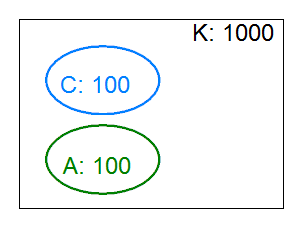
\includegraphics[scale=0.3] {img/table-img1.png}}
& 
\begin{tabular}{l l}accuracy& 0\%\\\\ recall & 0\%\end{tabular}
& 0 \% & 0 \% & 0 \% & 0 \% \\ \hline 

\raisebox{-.5\height}{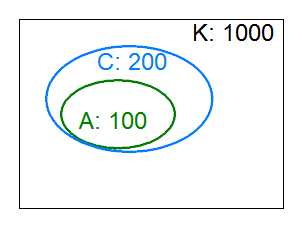
\includegraphics[scale=0.3] {img/table-img2.png}}
&
\begin{tabular}{l l}accuracy& 50\%\\\\ recall & 100\%\end{tabular}
& 0 \% & 0 \% & 0 \% & 0 \% \\ \hline 

\raisebox{-.5\height}{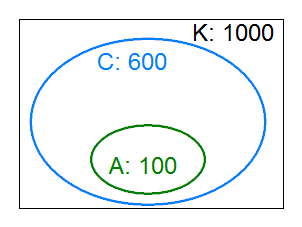
\includegraphics[scale=0.3] {img/table-img3.png}}
& 
\begin{tabular}{l l}accuracy& 16.7\%\\\\ recall & 100\%\end{tabular}
& 0 \% & 0 \% & 0 \% & 0 \% \\ \hline 


\raisebox{-.5\height}{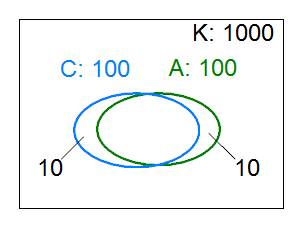
\includegraphics[scale=0.3] {img/table-img4.png}}
& 
\begin{tabular}{l l}accuracy& 90\%\\\\ recall & 90\%\end{tabular}
& 0 \% & 0 \% & 0 \% & 0 \% \\ \hline 

\raisebox{-.5\height}{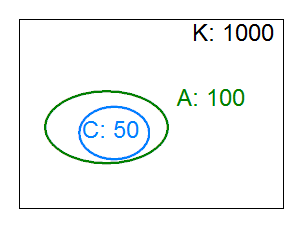
\includegraphics[scale=0.3] {img/table-img5.png}}
& 
\begin{tabular}{l l}accuracy& 50\%\\\\ recall & 100\%\end{tabular}
& 0 \% & 0 \% & 0 \% & 0 \% \\ \hline 

\end{tabular}
\end{table*}

%=====================================================================================
%=====================================================================================
%=====================================================================================
\subsection{Efficient heuristic computation}
- more

- more

- more



%=====================================================================================
%=====================================================================================
%=====================================================================================
\section{Evaluation Heuristics}
% Paper 1 
- more

- more

- more



%=====================================================================================
%=====================================================================================
%=====================================================================================
\section{Evaluation on Ontology Enrichment}
% Paper 2
- more

- more

- more


